\newpage
\section{Anhang}

    \subsection{Messwerte}
    \begin{figure}[H]
        \centering
        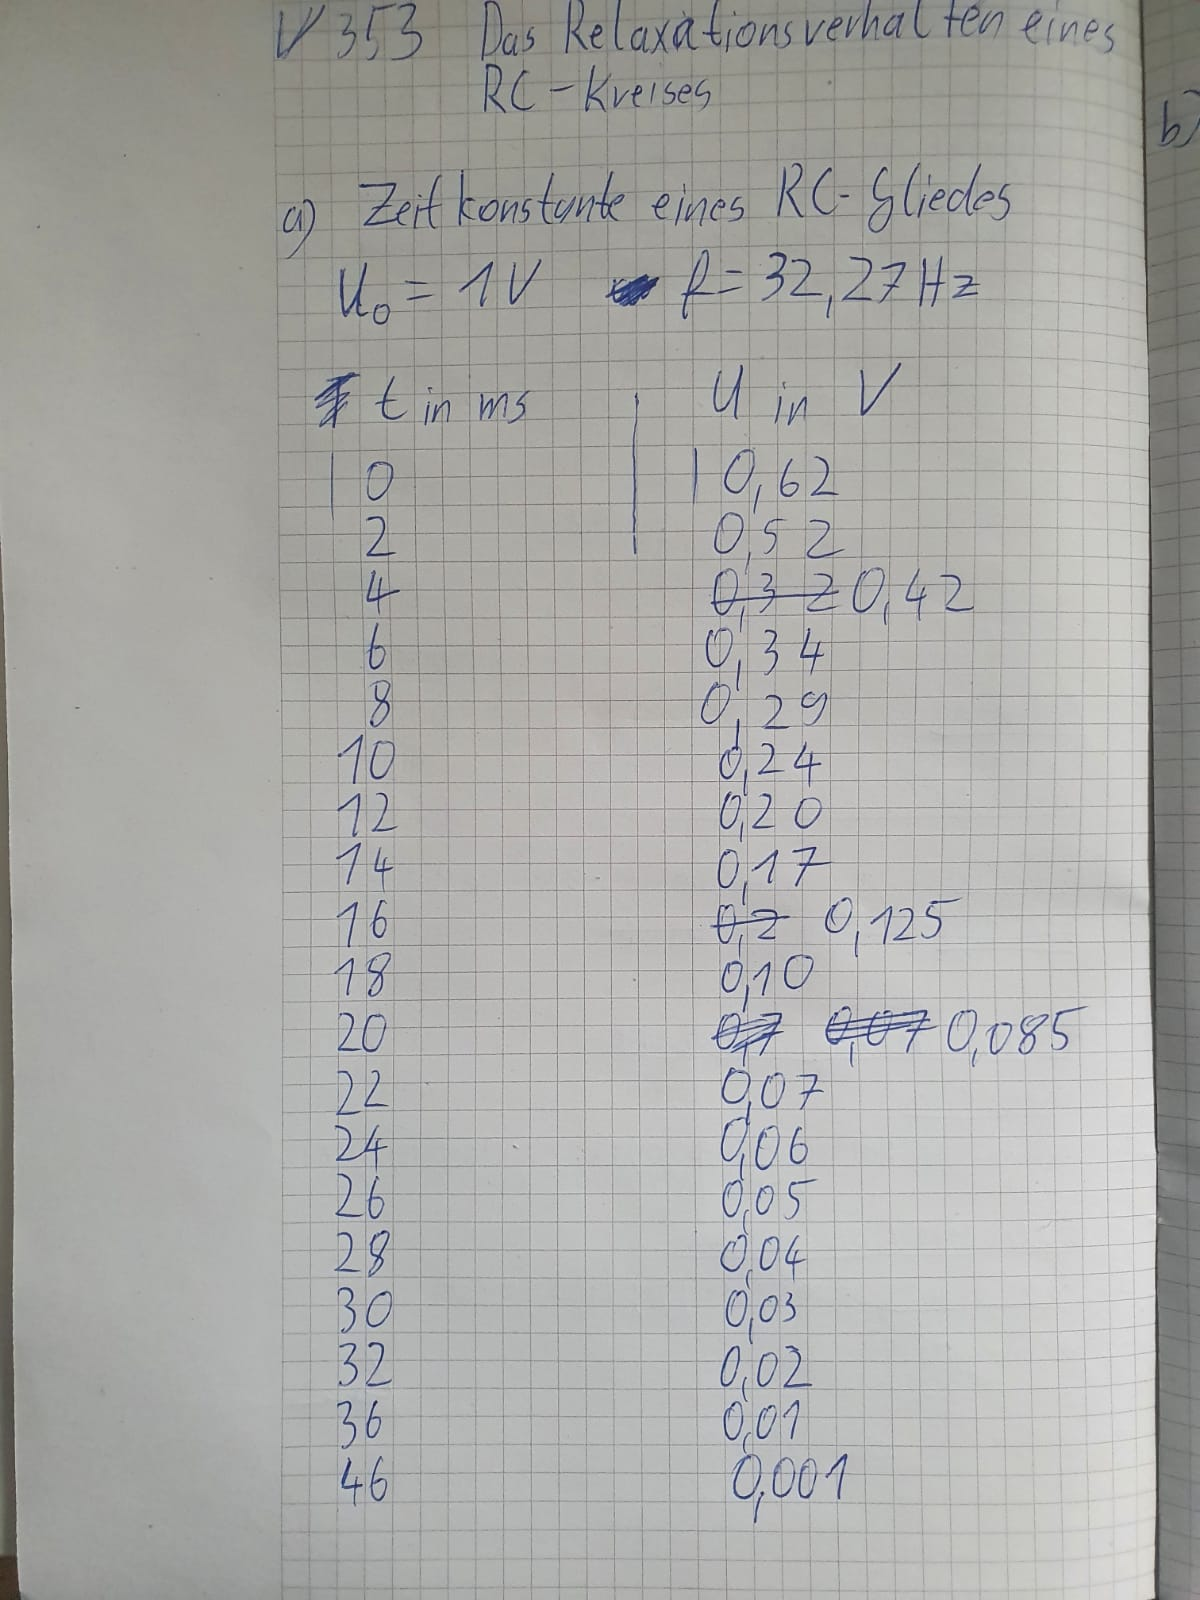
\includegraphics[width=0.63\textwidth]{latex/images/mess1.jpeg}
        \caption{Ein Foto der Messwerte im Protokollheft.}
        \label{img:mess1}
    \end{figure}

    \begin{figure}[H]
        \centering
        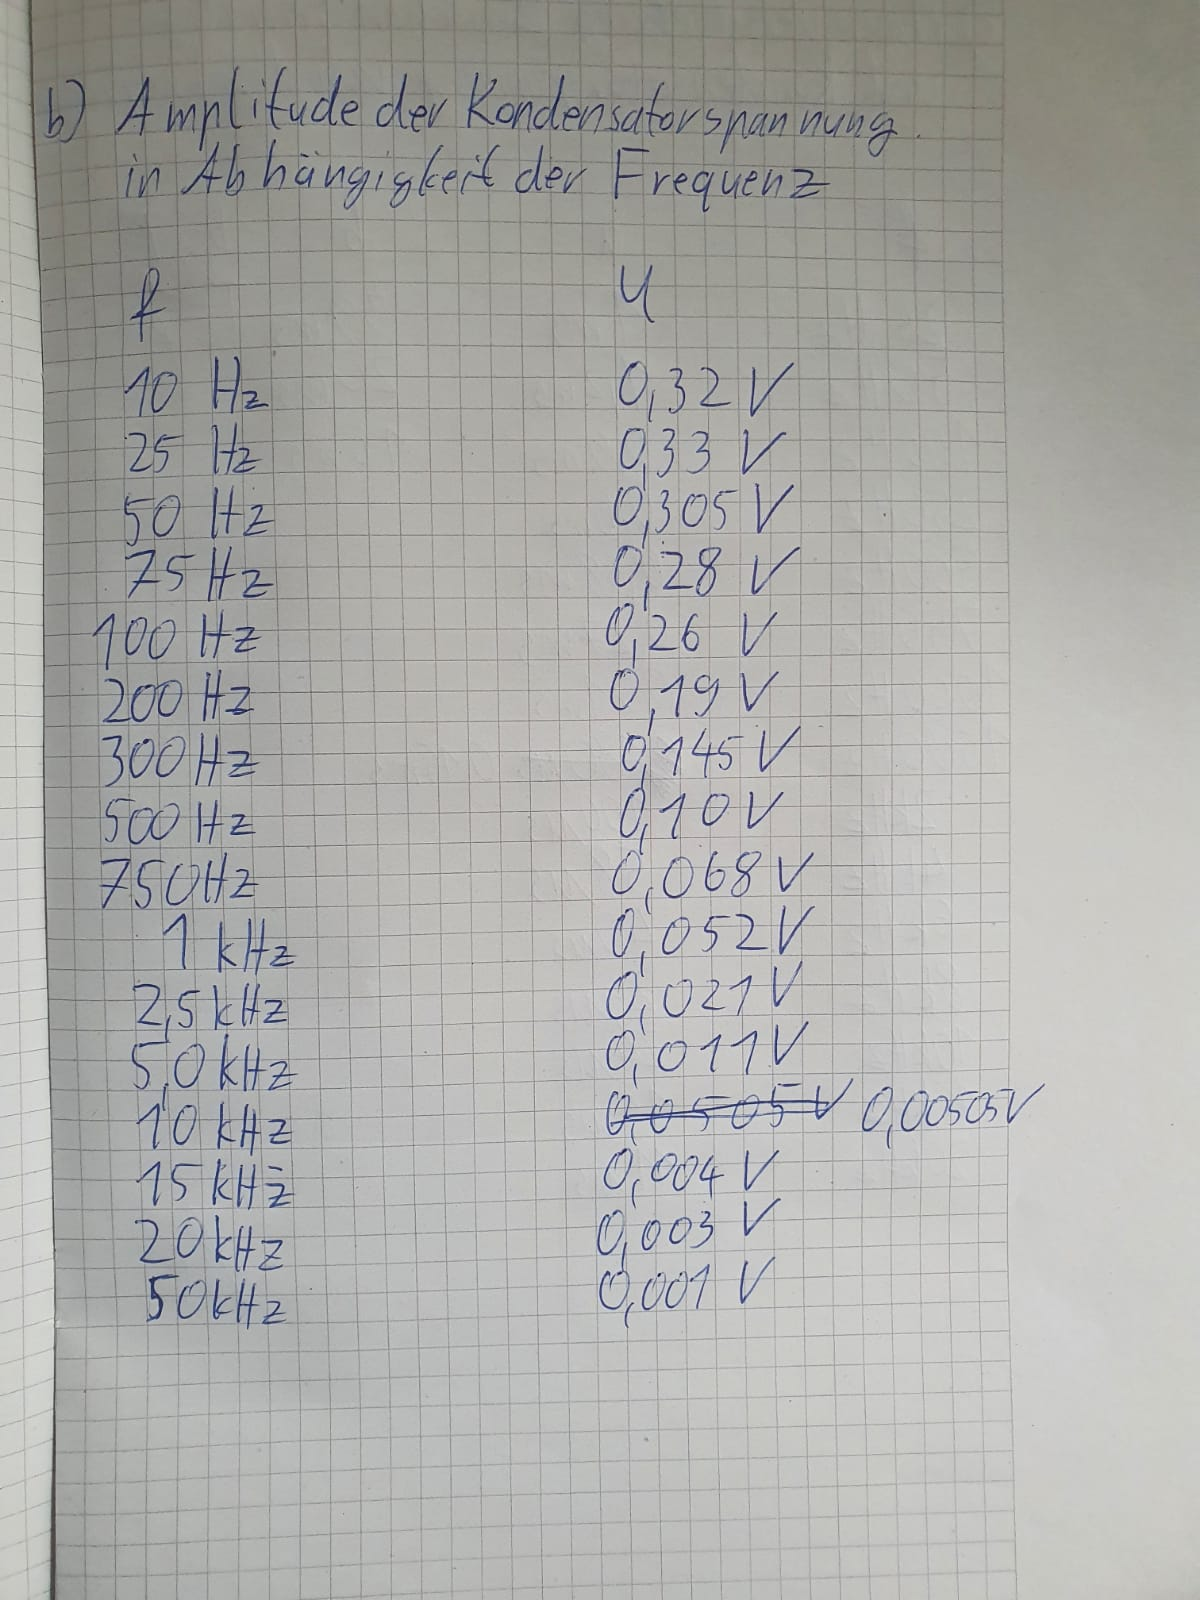
\includegraphics[width=0.63\textwidth]{latex/images/mess2.jpeg}
        \caption{Ein Foto der Messwerte im Protokollheft.}
        \label{img:mess2}
    \end{figure}


    \begin{figure}[H]
        \centering
        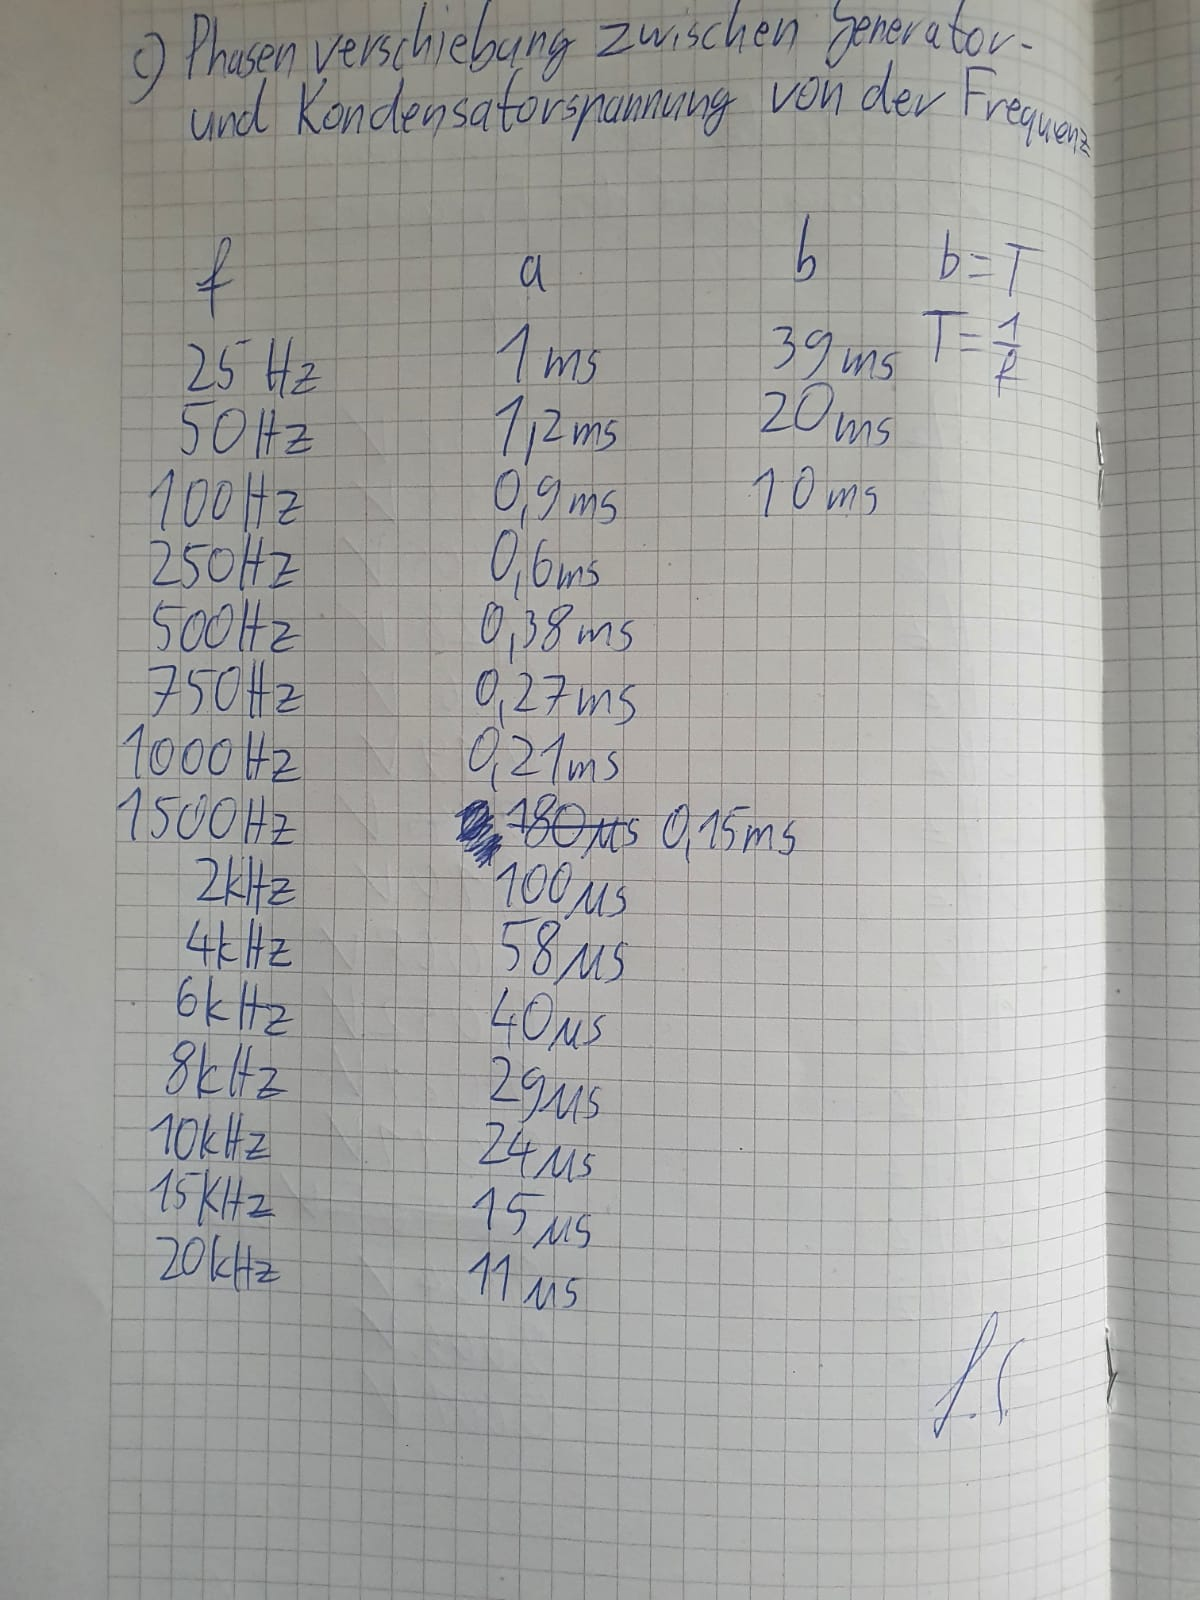
\includegraphics[width=0.63\textwidth]{latex/images/mess3.jpeg}
        \caption{Ein Foto der Messwerte im Protokollheft.}
        \label{img:mess3}
    \end{figure}





    \subsection{Aufbau}
    \begin{figure}[H]
        \centering
        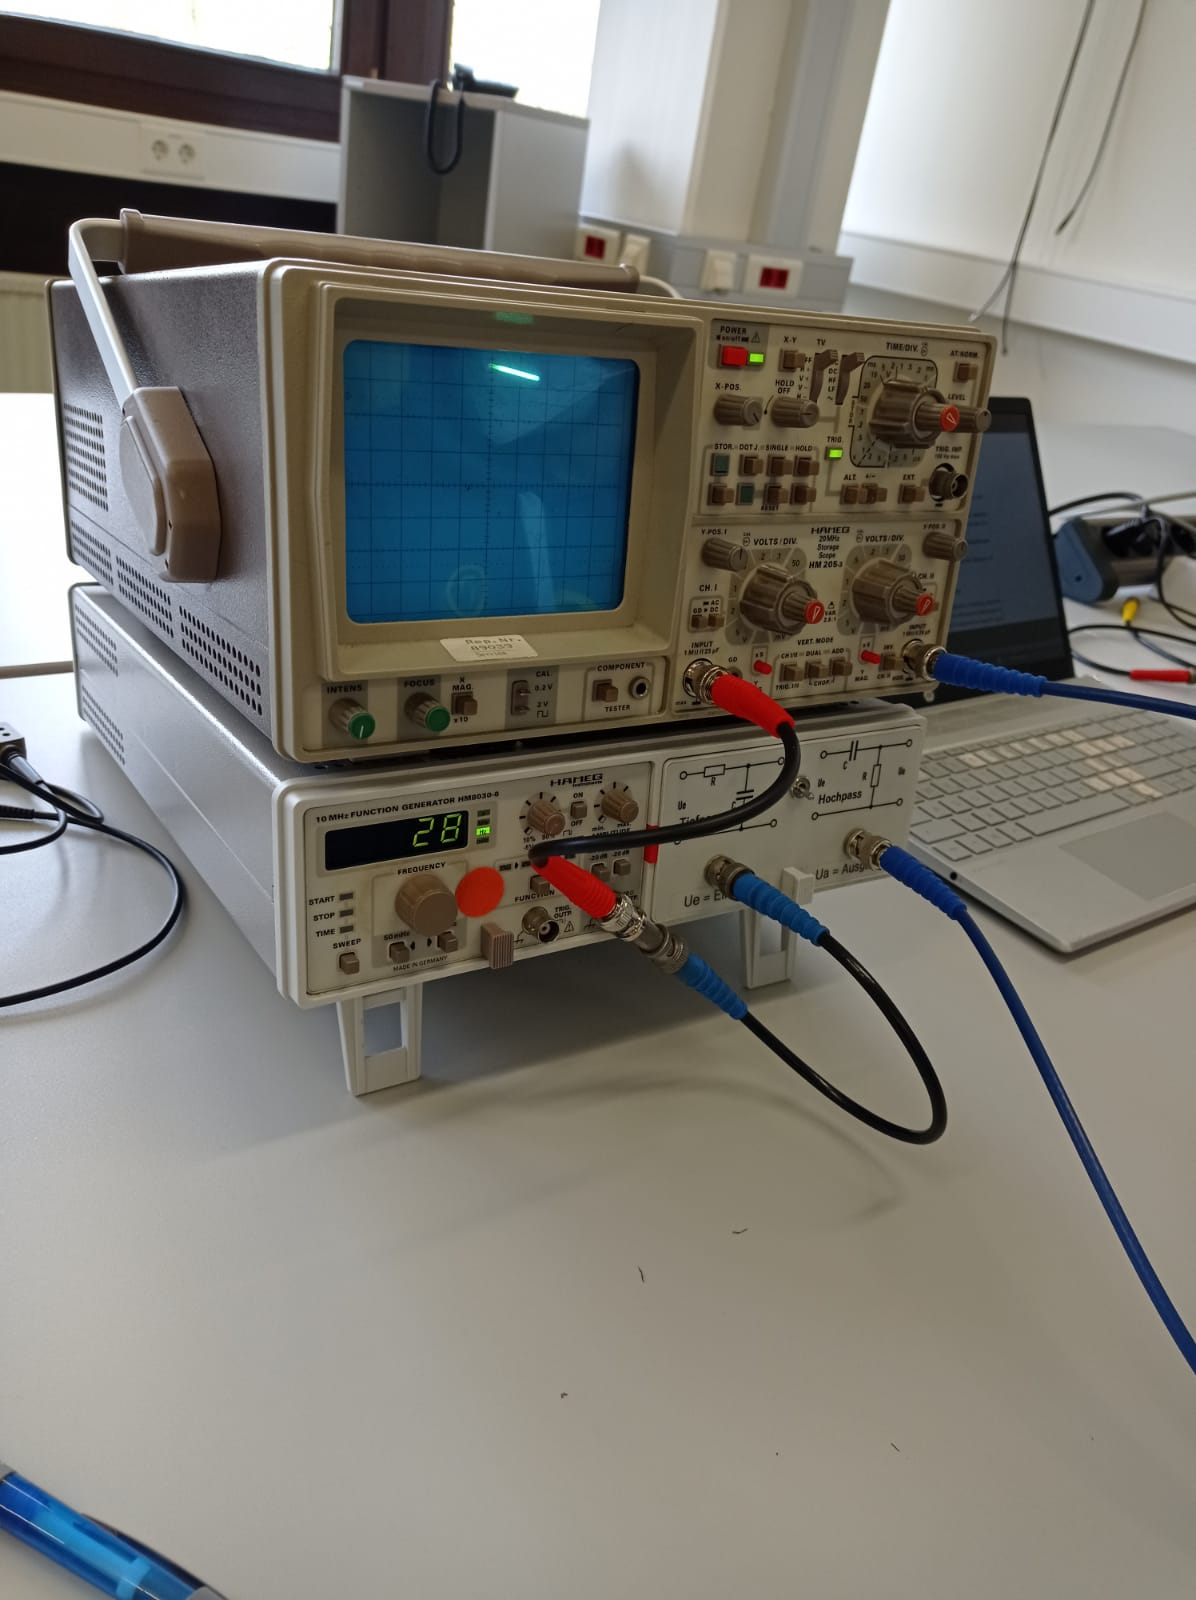
\includegraphics[width=0.63\textwidth]{latex/images/aufbau.jpeg}
        \caption{Ein Foto des Versuchsaufbaus.}
        \label{img:mess1}
    \end{figure}
